\chapter{Curvas en $\realR^{3}$}\label{ch:curvas-en-r3}

En este capítulo daremos una primera definición de \emph{curva}, con la cual trabajaremos
a lo largo de esta sección. En el siguiente capítulo daremos una definición más general.
Veremos como calcular el vector tangente a la curva y como encontrar su espacio tangente.

Es importante mencionar que aunque nuestros casos serán para $\realR^{3}$ son totalmente
válidos para $\realR^{2}$.

\section{¿Qu\'e es una curva?}

Si nos pidieran dar un ejemplo de una curva, podriamos decir que una l\'inea recta, como
$y-2x=1$ (aunque no sea \emph{curva}), o un c\'irculo, por ejemplo $x^{2} + y^{2} = 1$, 
o tal vez una par\'abola, $y-x^{2}=0$.

Todas estas curvas est\'an descritas por su ecuaci\'on cartesiana
$$ f(x,y) = c \text{,} $$
donde $f$ es una funci\'on de $x$ y $y$ y $c$ es constante. Todos estos ejemplos son curvas
en $\realR^{2}$, pero podr\'iamos considerar curvas en $\realR^{3}$ tambi\'en, por ejemplo
el eje $x$ en $\realR^{3}$ es la l\'inea recta dada por
$$y=0\text{,} \quad z=0 \text{,}$$
y de forma general una curva en $\realR^{3}$ se puede definir con el par de ecuaciones
$$ f(x,y,z)=c_{1}\text{,}\quad f(x,y,z)=c_{2} \text{,}$$
curvas de \'este estilo son llamadas \emph{curvas de nivel}.

Pero existe una forma diferente de pensar las curvas que nos ayudar\'a en muchas ocasiones.
Podemos ver a una curva como la trayectoria recorrida por un punto en movimiento. As\'i
$c(t)$, es la posici\'on del punto en el tiempo $t$. Usaremos esta idea para dar nuestra
primera definici\'on formal de curva en $\realR^{3}$

\begin{definition}
    Una curva parametrizada en $\realR^{3}$ es una mapeo $c:(\alpha,\beta) \rightarrow \realR^{3}$,
    para alg\'un $\alpha$, $\beta$ con $-\infty \le \alpha < \beta \le \infty$.
\end{definition}

\begin{myExample}
    Una línea recta es el tipo más simple de \emph{curva} en el espacio Euclideo. Es una curva
    $c:\realR \rightarrow \realR^{3}$ tal que
    $$ c(t) = p + tq$$
    Donde $p$,$q$ $\in \realR^{3}$
\end{myExample}

\begin{myExample}
    La curva (hélice) $t \rightarrow (a\cos{t},a\sin{t},0)$ viaja alrededor de un círculo de 
    $a > 0$ en el plano $xy$ de $\realR^{3}$. Si dejamos que la curva suba a baje de manera
    uniforme, obtenemos la hélice $c:\realR \rightarrow \realR^{3}$, dada por
    $$ c(t) = (a\cos{t}, a\sin{t}, bt) $$
    donde $a>0$, $b \ne 0$
\end{myExample}

\begin{figure}[!ht]
  \begin{center}
      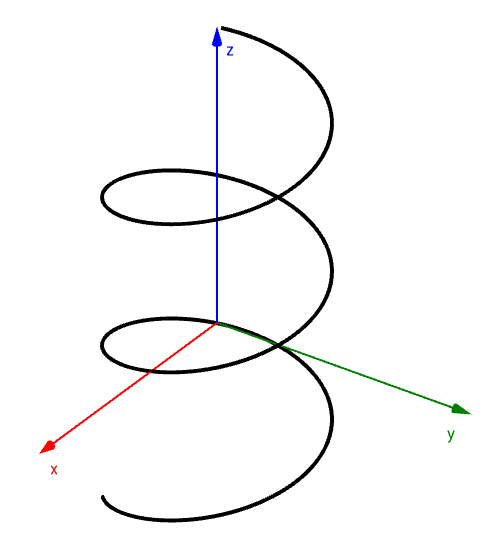
\includegraphics[width=0.6\linewidth]{gfx/helice}
      \caption{Hélice}
      \label{fig:boat1}
  \end{center}
\end{figure}

Estas curvas estar\'an descritas exclusivamente en t\'erminos de funciones \emph{suaves}: una funci\'on
$f:(\alpha,\beta) \rightarrow \realR$ se dice que es \emph{suave} si sus derivadas $\frac{d^{n}f}{dt^{n}}$
existen para todo $n \ge 1$.

Para diferenciar una \emph{funci\'on vectorial} como $c(t)$, diferenciamos componente a componente, si
$$ c(t) = (c_{1}(t),c_{2}(t),c_{3}(t))\text{,}$$
entonces
$$ \frac{dc}{dt} = \left( \frac{dc_{1}}{dt},\frac{dc_{2}}{dt},\frac{dc_{3}}{dt}\right)\text{.}$$

De aqu\'i en adelante todas las curvas parametrizadas en este texto se asumiran suaves.

\section{Vector tangente a una curva parametrizada}

\begin{definition}
    Si $c$ es una curva parametrizada, su primera derivada $c'(t)$ es llamada el vector tangente
    de $c$ en el punto $c(t)$.
\end{definition}

\begin{myExample}
    El caracol de Pascal es la curva parametrizada
    $$ c(t)=((1+2\cos{t})\cos{t},(1+2\cos{t}+2\cos{t})\text{,} \quad t \in \realR$$
    El vector tangente es
    $$ c'(t)=(-\sin{t}-2\sin{2t},\cos{t}+2\cos{2t})$$
    En particular,
    $$ c'(2\pi/3) = (\sqrt{3}/2,-3/2)$$
\end{myExample}

\begin{figure}[!ht]
  \begin{center}
      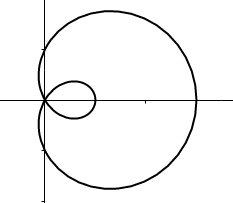
\includegraphics[width=0.7\linewidth]{gfx/limacon2}
      \caption{Curva de Pascal}
      \label{fig:boat1}
  \end{center}
\end{figure}


Esta definición puede ser interpretada geometricamente de la siguiente forma. La derivada en
$t$ de la función de valor real $f$ en $\realR$ esta dada por

$$ \frac{df}{dt}(t) = \lim_{h \rightarrow 0} \frac{f(t+h)-f(t)}{h} $$

Esta expresión también tiene sentido si remplazamos $f$ por una curva $c = (c_{1},c_{2},c_{3})$,
es decir,

$$ \frac{1}{h}(c(t+h)-c(t)) =$$
$$\left( \frac{c_{1}(t+h)-c_{1}(t)}{h},\frac{c_{2}(t+h)-c_{2}(t)}{h},\frac{c_{3}(t+h)-c_{3}(t)}{h} \right) $$

Este es el vector $c(t)$ hacia $c(t+h)$, multiplicado escalarmente por $\frac{1}{h}$. Ahora, cuando $h$ se hace
muy pequeño, $c(t+h)$ se aproxima a $c(t)$ y en el límite $h \rightarrow 0$, obtenemos el vector tangente
$$\left( \frac{dc_{1}}{dt}(t),\frac{dc_{2}}{dt}(t),\frac{dc_{3}}{dt}(t) \right) $$
el cual tiene como punto inicial $c(t)$.

\section{Espacio tangente a una curva parametrizada}

Sabemos que dados un punto $p$ y una direcci\'on $u$ podemos describir parametricamente una
l\'inea recta que contenga a $p$ con direcci\'on de $u$ (paralela a $u$) de la forma
$$ l(t) = p + tu \text{,} \quad t \in \realR \text{.}$$

Tomaremos esta idea para definir el \emph{espacio tangente} a una curva.

\begin{definition}
    Si $c(t)$ es una curva parametrizada, entonces el espacio tangente (recta tangente) a $c(t)$ es
    $$ l(t_{1}) = ( c(t) + t_{1}c'(t) ) \text{,} \quad t_{1} \in \realR \text{.}$$
\end{definition}

\begin{myExample}
    Tomando el ejemplo 3.4, el espacio tangente (recta tangente) en $c(\pi/4)$ es
    $$ l(t_{1}) = (c(\pi/4) + t_{1}c'(\pi/4)) $$
\end{myExample}

\begin{figure}[!ht]
  \begin{center}
      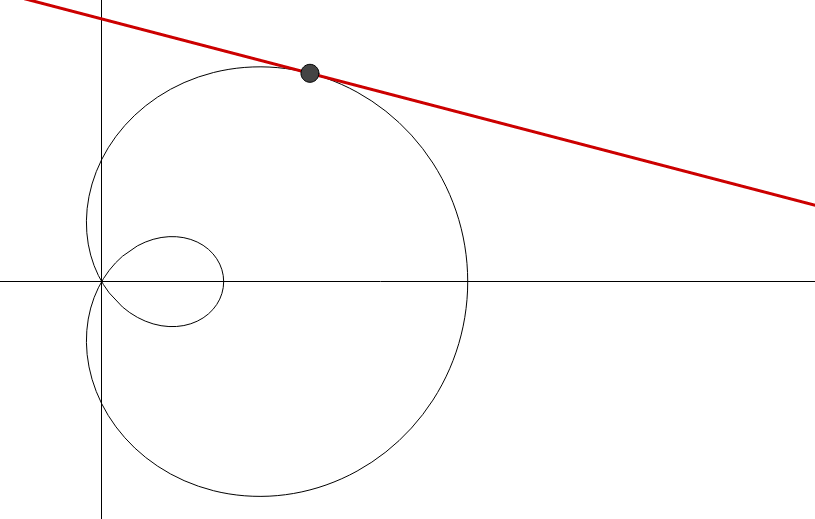
\includegraphics[width=0.8\linewidth]{gfx/limacon}
      \caption{Espacio tangente a la curva de Pascal $c$ en $c(\pi/4)$}
      \label{fig:boat1}
  \end{center}
\end{figure}


